\documentclass[aspectratio=169,hyperref={pdfpagelabels=false}]{beamer}
\setbeameroption{show notes}

\usepackage{helvet}
\usepackage[english]{babel}
\usepackage{pgfplots}
\usepackage{pgf}
\pgfplotsset{compat=newest}
\usepackage{booktabs}
\usepackage[T1]{fontenc}
\usepackage[utf8]{inputenc}
\usepackage{lipsum}
\usepackage{tcolorbox}
\usepackage{xcolor}
\usepackage{listings}
\usepackage[nopatch=footnote]{microtype}
\usepackage{float}
\usepackage{siunitx}
\usepackage{multicol}
%\usepackage{hyperref}
\usepackage{dsfont}
\usepackage{caption}
\usepackage{subcaption}

% Colours! 
\newcommand{\targetcolourmodel}{cmyk} % rgb for a digital version, cmyk for a printed version. Only use lowercase
\selectcolormodel{\targetcolourmodel}

% Define colours from https://www.designguide.dtu.dk/
\definecolor{dtured}    {rgb/cmyk}{0.6,0,0 / 0,0.91,0.72,0.23}
\definecolor{blue}      {rgb/cmyk}{0.1843,0.2431,0.9176 / 0.88,0.76,0,0}
\definecolor{brightgreen}{rgb/cmyk}{0.1216,0.8157,0.5098 / 0.69,0,0.66,0}
\definecolor{navyblue}  {rgb/cmyk}{0.0118,0.0588,0.3098 / 1,0.9,0,0.6}
\definecolor{yellow}    {rgb/cmyk}{0.9647,0.8157,0.3019 / 0.05,0.17,0.82,0}
\definecolor{orange}    {rgb/cmyk}{0.9882,0.4627,0.2039 / 0,0.65,0.86,0}
\definecolor{pink}      {rgb/cmyk}{0.9686,0.7333,0.6941 / 0,0.35,0.26,0}
\definecolor{grey}      {rgb/cmyk}{0.8549,0.8549,0.8549 / 0,0,0,0.2}
\definecolor{red}       {rgb/cmyk}{0.9098,0.2471,0.2824 / 0,0.86,0.65,0}
\definecolor{green}     {rgb/cmyk}{0,0.5333,0.2078 / 0.89,0.05,1,0.17}
\definecolor{purple}    {rgb/cmyk}{0.4745,0.1373,0.5569 / 0.67,0.96,0,0}

\newcommand{\dtulogocolour}{white} % Colour of the DTU logo: white, black or dtured
\newcommand{\frontpagetextcolour}{white} % front page text colour: white or black
\colorlet{frontbackcolor}{blue} % Set the background colour of the front- and back page. Choose the colour so it matches the main colour of front page picture

% DTU colours for diagrams
% You might want to make the front/back page background colour the first colour in the plot cycle list.
\pgfplotscreateplotcyclelist{DTU}{%
dtured,         fill=dtured,        \\%
blue,           fill=blue,          \\%
brightgreen,    fill=brightgreen    \\%
navyblue,       fill=navyblue       \\%
yellow,         fill=yellow         \\%
orange,         fill=orange         \\%
grey,           fill=grey           \\%
red,            fill=red            \\%
green,          fill=green          \\%
purple,         fill=purple         \\%
}


% Font
% There is no corporate serif font in the DTU design guide. The DTU design team has proposed to use Neo Sans for headings - and Arial for the body text.
% To change heading font to NeoSans Pro please upload both NeoSansPro-Regular.otf and NeoSansPro-Medium.otf to the root directory.
\setmainfont{Arial}
\renewcommand\thepart{Part \Roman{part}}
\IfFontExistsTF{NeoSansPro-Medium.otf}
{ %If True set headings to NeoSans Pro
\newfontface\NeoSansProReg{NeoSansPro-Regular.otf}
\newfontface\NeoSansProMed{NeoSansPro-Medium.otf}
\titleformat{\part}[display]{\NeoSansProMed \huge \centering}{\NeoSansProMed \Huge \thepart}{1em}{\thispagestyle{empty}}{}
\titleformat{\chapter}{\NeoSansProMed\huge}{\thechapter}{1em}{\raggedright}
\titleformat{\section}{\NeoSansProMed\Large}{\thesection}{1em}{\raggedright}
\titleformat{\subsection}{\NeoSansProMed\large}{\thesubsection}{1em}{\raggedright}
\titleformat{\subsubsection}{\NeoSansProMed\normalsize}{\thesubsubsection}{1em}{\raggedright}
\newcommand\TitleFont[1]{{\NeoSansProMed #1}}
\newcommand\titlefont[1]{{\NeoSansProReg #1}}
}
{ % If false
\titleformat{\part}[display]{\bfseries\huge \centering}{\bfseries\Huge \thepart}{1em}{\thispagestyle{empty}}{}
\titleformat{\chapter}{\bfseries\huge}{\thechapter}{1em}{\raggedright}
\titleformat{\section}{\bfseries\Large}{\thesection}{1em}{\raggedright}
\titleformat{\subsection}{\bfseries\large}{\thesubsection}{1em}{\raggedright}
\titleformat{\subsubsection}{\bfseries\normalsize}{\thesubsubsection}{1em}{\raggedright}
\newcommand\TitleFont[1]{{\bfseries #1}}
\newcommand\titlefont[1]{{#1}}
}
\urlstyle{sf}
%\def\UrlFont{\NeoSansProReg}


% If you wish to use the pdflatex compiler, sans-serif Helvetica can be used as a replacement for Arial. In this way you will be able to use the microtype package. Remember to add \usepackage[utf8]{inputenc} and disable the fontspec package. 
%\newcommand\TitleFont[1]{{\bfseries #1}}
%\newcommand\titlefont[1]{{#1}}
%\fontfamily{qhv}\selectfont
%\renewcommand{\familydefault}{\sfdefault}


% Watermark for confidential or draft (or anything else)
%\sffamily % set the correct font for the watermark
%%\newsavebox\mybox
%%\savebox\mybox{\tikz[color=grey,opacity=0.5]\node{Template};}

%%\newwatermark*[
%%  oddpages,
%%  angle=60,
%%  scale=12,
%%  %fontfamily=qhv,
%%  xpos=-40,
%%  ypos=30,
%%]{\usebox\mybox}

%%\newwatermark*[
%%  evenpages,
%%  angle=60,
%%  scale=12,
%%  %fontfamily=qhv,
%%  xpos=-50,
%%  ypos=30,
%%]{\usebox\mybox}


% Table of contents (TOC) and numbering of headings
\setcounter{tocdepth}{1}    % Depth of table of content: sub sections will not be included in table of contents
\setcounter{secnumdepth}{2} % Depth of section numbering: sub sub sections are not numbered

\makeatletter % Reset chapter numbering for each part
\@addtoreset{chapter}{part}
\makeatother  

% Spacing of titles and captions
\titlespacing\chapter{0pt}{0pt plus 4pt minus 2pt}{4pt plus 2pt minus 2pt}
\titlespacing\section{0pt}{12pt plus 3pt minus 3pt}{2pt plus 1pt minus 1pt}
\titlespacing\subsection{0pt}{8pt plus 2pt minus 2pt}{0pt plus 1pt minus 1pt}
\titlespacing\subsubsection{0pt}{4pt plus 1pt minus 1pt}{-2pt plus 1pt minus 1pt}
\captionsetup{belowskip=\parskip,aboveskip=4pt plus 1pt minus 1pt}

% Setup header and footer
\fancypagestyle{main}{% All normal pages
    \fancyhead{}
    \fancyfoot{}
    \renewcommand{\headrulewidth}{0pt}
    \fancyfoot[LE,RO]{\footnotesize \thepage}
    \fancyfoot[RE,LO]{\footnotesize \thesistitle} % - \rightmark
    \fancyhfoffset[E,O]{0pt}
}
\fancypagestyle{plain}{% Chapter pages
    \fancyhead{}
    \fancyfoot{}
    \renewcommand{\headrulewidth}{0pt}
    \fancyfoot[LE,RO]{\footnotesize \thepage}
    \fancyfoot[RE,LO]{\footnotesize \thesistitle} % - \leftmark
    \fancyhfoffset[E,O]{0pt}
}


% Setup for diagrams and graphs (tikz images) 
\usetikzlibrary{spy}    % For magnifying anything within a tikzpicture, see the line graph
\usepgfplotslibrary{statistics} % Package for the boxplot
\pgfplotsset{ % Setup for diagrams
compat=newest,
major x grid style={line width=0.5pt,draw=grey},
major y grid style={line width=0.5pt,draw=grey},
legend style={at={(0.5,-0.1)}, anchor=north,fill=none,draw=none,legend columns=-1,/tikz/every even column/.append style={column sep=10pt}},
axis line style={draw=none},
tick style={draw=none},
every axis/.append style={ultra thick},
tick label style={/pgf/number format/assume math mode}, % To apply main font to tick labels (numbers on the axis)
}
\tikzset{every mark/.append style={scale=1.5}}


% Hypersetup
\hypersetup{
    pdfauthor={\thesisauthor},
    pdftitle={\thesistitle},
    pdfsubject={\thesissubtitle},
    pdfdisplaydoctitle,
    bookmarksnumbered=true,
    bookmarksopen,
    breaklinks,
    linktoc=all,
    plainpages=false,
    unicode=true,
    colorlinks=false,
    hidelinks,                        % Do not show boxes or coloured links.
}


% Listings setup
\lstset{
    basicstyle=\footnotesize\ttfamily,% the size of the fonts that are used for the code
    commentstyle=\color{green},       % comment style
    keywordstyle=\bfseries\ttfamily\color{blue}, % keyword style
    numberstyle=\sffamily\tiny\color{grey}, % the style that is used for the line-numbers
    stringstyle=\color{purple},       % string literal style
    rulecolor=\color{grey},           % if not set, the frame-color may be changed on line-breaks within not-black text (e.g. comments (green here))
    breakatwhitespace=false,          % sets if automatic breaks should only happen at whitespace
    breaklines=true,                  % sets automatic line breaking
    captionpos=b,                     % sets the caption-position to bottom
    deletekeywords={},                % if you want to delete keywords from the given language
    escapeinside={\%*}{*)},           % if you want to add LaTeX within your code
    frame=single,                     % adds a frame around the code
    xleftmargin=4pt, 
    morekeywords={*,...},             % if you want to add more keywords to the set
    numbers=left,                     % where to put the line-numbers; possible values are (none, left, right)
    numbersep=10pt,                   % how far the line-numbers are from the code
    showspaces=false,                 % show spaces everywhere adding particular underscores; it overrides 'showstringspaces'
    showstringspaces=false,           % underline spaces within strings only
    showtabs=false,                   % show tabs within strings adding particular underscores
    stepnumber=1,                     % the step between two line-numbers. If it's 1, each line will be numbered
    tabsize=2,                        % sets default tabsize to 2 spaces
    title=\lstname,                   % show the filename of files included with \lstinputlisting; also try caption instead of title
}

% Signature field
\newlength{\myl}
\newcommand{\namesigdatehrule}[1]{\par\tikz \draw [black, densely dotted, very thick] (0.04,0) -- (#1,0);\par}
\newcommand{\namesigdate}[2][]{%
\settowidth{\myl}{#2}
\setlength{\myl}{\myl+10pt}
\begin{minipage}{\myl}%
\begin{center}
    #2  % Insert name from the command eg. \namesigdate{\authorname}
    \vspace{1.5cm} % Spacing between name and signature line 
    \namesigdatehrule{\myl}\smallskip % Signature line and a small skip
    \small \textit{Signature} % Text under the signature line "Signature"
    \vspace{1.0cm} % Spacing between "Signature" and the date line
    \namesigdatehrule{\myl}\smallskip % Date line and a small skip
    \small \textit{Date} % Text under date line "Date" 
\end{center}
\end{minipage}
}

% For the back page: cleartoleftpage
\newcommand*\cleartoleftpage{%
  \clearpage
  \ifodd\value{page}\hbox{}\newpage\fi
}


\newcommand{\setcolor}[1]{\def\chosencolor{#1}}
\newcommand{\setdepartment}[1]{\def\department{#1}}

\usetheme{DTU}
\setbeamersize{text margin left=22mm}
\def\insertframetitle{}

\newcommand{\inserttitlepage}{
    \begin{frame}[plain, noframenumbering]{}

        \begin{center}
            \hspace{-3.6em}
            \includegraphics[width = 0.25\paperwidth]{logos/\targetcolourmodel/white.pdf}
        \end{center}

    \end{frame}

    \begin{frame}[plain]{}
        \color{white}\maketitle
    \end{frame}

    \setbeamercolor{background canvas}{bg = white}
}


\newcommand{\documenttype}{Master Thesis}
\newcommand{\thesistitle}{Clusters in SAE Latents}
\newcommand{\thesissubtitle}{Characterizing Sparse Autoencoder Latents for LLM Interpretability}

\newcommand{\thesisauthor}{Albert Ramus Sidenius Garde} % Your name :) 
\newcommand{\studentnumber}{s183969}
\newcommand{\thedate}{\today} % For example "June, 2019"

\newcommand{\thesisdepartment}{DTU Compute}
\newcommand{\departmentdescriber}{Department of Civil Engineering}
\newcommand{\addressI}{Brovej, Building 118}
\newcommand{\addressII}{2800 Kgs. Lyngby}
\newcommand{\departmentwebsite}{www.byg.dtu.dk}

\usepackage[utf8]{inputenc}
\usepackage{fullpage}

% Stop Vincents stupid indryk ved at sætte længden af dem til 0
\setlength\parindent{0pt}

% Selectively silence warnings
\usepackage{silence}
\WarningFilter{hyperref}{Token not allowed}

% Math notation
\usepackage{amsmath}
\usepackage{amssymb}
\usepackage{amsfonts}
\usepackage{amsthm}
\usepackage{mathrsfs}
\usepackage{bm} % Used for bold math

% Subscript before
\usepackage{tensor}

% Framing
\usepackage{tcolorbox}
\tcbuselibrary{theorems}

% Placement of figures
\usepackage{float}

% Figures
\usepackage{graphicx}
\usepackage{subfig}

% Pseudocode
\usepackage{algorithmic}

% Enumerations
\usepackage{enumitem}

% Potter proof!
\usepackage{stmaryrd}

% Units
\usepackage{siunitx}

% Todos
\usepackage{todonotes}

% Hyperref
\usepackage[hidelinks]{hyperref}

% More complex arguments
\usepackage{xparse}

% Bibliography
\usepackage[authoryear]{natbib}

% Symbols
%% Arabic symbols
\usepackage{arabtex}
\setarab
\arabtrue

\newcommand{\arj}{\RL{j}}
\newcommand{\ark}{\RL{.k}}
\newcommand{\artea}{\RL{.s}}
\newcommand{\ardoublemu}{\RL{s}}
\newcommand{\arsmiley}{\RL{t}}
\newcommand{\arhandcuffs}{\RL{mh}}

%% Standard symbols
\newcommand{\e}{\mathrm{e}}
\newcommand{\im}{\mathrm{i}}
\newcommand{\diff}{\mathrm{d}}
\newcommand{\id}{\mathrm{id}}
\renewcommand{\R}{\mathbb{R}}
\newcommand{\C}{\mathbb{C}}
\newcommand{\N}{\mathbb{N}}
\newcommand{\Z}{\mathbb{Z}}
\newcommand{\F}{\mathbb{F}}
\newcommand{\M}{\mathbb{M}}
\newcommand{\xor}{\oplus}


% Theorem boxes
\newcommand{\ksjlcisavbff}{ksjlcisavbff}


\newtcbtheorem{theorem}{Theorem}%
{colframe=black,fonttitle=\bfseries,
separator sign={\ -}}{theorem}
\newtcbtheorem[use counter from=theorem]{lemma}{Lemma}%
{colframe=black,fonttitle=\bfseries,
separator sign={\ -}}{lemma}
\newtcbtheorem[use counter from=theorem]{corollary}{Corollary}%
{colframe=black,fonttitle=\bfseries,
separator sign={\ -}}{corollary}
\newtcbtheorem[use counter from=theorem]{definition}{Definition}%
{colframe=black,fonttitle=\bfseries,
separator sign={\ -}}{definition}
\newtcbtheorem[use counter from=theorem]{example}{Example}%
{colframe=black,fonttitle=\bfseries,
separator sign={\ -}}{example}
\newtcbtheorem[use counter from=theorem]{problem}{Problem}%
{colframe=black,fonttitle=\bfseries,
separator sign={\ -}}{problem}

%\newmdtheoremenv[nobreak=true]{theorem}{Theorem}
%\newmdtheoremenv[nobreak=true]{lemma}{Lemma}
%\newmdtheoremenv[nobreak=true]{corollary}{Corollary}
%\newmdtheoremenv[nobreak=true]{definition}{Definition}
%\newmdtheoremenv[nobreak=true]{problem}{Problem}
%\newmdtheoremenv{example}{Example}

% Symbol formatting
\renewcommand{\vec}[1]{\mathbf{#1}}
\newcommand{\mat}[1]{\mathbf{#1}}
\newcommand{\set}[1]{\mathcal{#1}}

% Vector span
\newcommand{\vspan}{\mathrm{span}}

% Column vectors
\makeatletter
\newcommand{\cvec}[1]{
    \left[\begin{array}{c}#1\cvecchecknextarg}
\newcommand{\cvecchecknextarg}{\@ifnextchar\bgroup{\cvecgobblenextarg}{\end{array}\right]}}
\newcommand{\cvecgobblenextarg}[1]{\\#1\@ifnextchar\bgroup{\cvecgobblenextarg}{\end{array}\right]}}
\makeatother

% Row vectors
\makeatletter
\newcommand{\rvec}[2]{
    \left[\begin{array}{*{#1}{c}}#2\rvecchecknextarg}
\newcommand{\rvecchecknextarg}{\@ifnextchar\bgroup{\rvecgobblenextarg}{\end{array}\right]}}
\newcommand{\rvecgobblenextarg}[1]{&#1\@ifnextchar\bgroup{\rvecgobblenextarg}{\end{array}\right]}}
\makeatother

% Vertical iff
\newcommand{\viff}{\Updownarrow}

% Absolute
\newcommand{\abs}[1]{\left\lvert#1\right\lvert}

% Norm
\newcommand{\norm}[1]{\left\lvert\left\lvert#1\right\lvert\right\lvert}

% Inner product
\newcommand{\iprod}[2]{\left\langle#1,#2\right\rangle}

% Complex conjugate
\newcommand{\conj}[1]{\overline{#1}}

% Transpose
\newcommand{\trans}[1]{#1^\top}

% Conjugate transpose (adjunct)
\newcommand{\adj}[1]{#1^*}

% Infinite sum
\newcommand{\infsum}[2][1]{\sum_{#2=#1}^\infty}

% Label specific row in align
\newcommand\numberthis[1]{\stepcounter{equation}\label{#1}\tag{\theequation}}

% Conditional probability
\newcommand\given[1][]{\:#1\vert\:}

% Contradiction
\newcommand{\contradiction}{\ensuremath{\lightning}}

% Closure
\newcommand{\closure}[1]{\overline{#1}}

% Matrix trace
\newcommand{\trace}{\mathrm{tr}}

% Map image
\DeclareMathOperator{\ima}{im}

% Kronecker product	
\newcommand{\kronprod}{\otimes}

% Direct sum
\newcommand{\dirsum}{\oplus}

% Element-wise product
\newcommand{\elemprod}{\circ}
 
% Matrix representation of linear operator in basis
\newcommand{\linopbasis}[3]{\tensor[_{#1}]{\left[#2\right]}{_{#3}}}

\newcommand{\powerset}[1]{\mathcal{P}\left(#1\right)}

\DeclareMathOperator*{\argmax}{arg\,max}
\DeclareMathOperator*{\argmin}{arg\,min}

% Remove numbers for headers
%\setcounter{secnumdepth}{-2}

% Image
\newcommand{\image}[3]{
    \begin{figure}[H]
        \centering
        \includegraphics[scale=#3]{#1} 
        \caption{#2}
    \end{figure}
} 

% Itemize characters
\renewcommand\labelitemii{\textbullet}
\renewcommand\labelitemiii{\textbullet}

\newcommand\matlist[2]{#1_1,#1_2,\dots,#1_{#2}}

% References a Theorem/Lemma/Corollary depending on the label (thr/lemma/cor).
% For example, if a label thr:hairy_ball exists, then \thref{hairy_ball} will evaluate to "Theorem \label{thr:hairy_ball}".
% If the theorem is later changed to a lemma, so thr:hairy_ball is renamed lemma:hairy_ball, \thref{hairy_ball} will instead evaluate to "\Lemma \label{lemma:hairy_ball}".
% What happens if two labels with the same name (both thr:hairy_ball and lemma:hairy_ball) is undefined.
\makeatletter
\newcommand\thref[1]{%
	\@ifundefined{r@theorem:#1}{%
		\@ifundefined{r@lemma:#1}{%
			\@ifundefined{r@corollary:#1}{%
				Definition \ref {definition:#1}%
			}{%
				Corollary \ref{corollary:#1}%
			}%
		}{%
			Lemma \ref{lemma:#1}%
		}%
	}{%
		Theorem \ref{theorem:#1}%
	}%
}
\makeatother


\title{\thesistitle}
\subtitle{\thesissubtitle}

\setdepartment{\thesisdepartment}
\setcolor{dtured}



\begin{document}
\inserttitlepage


\begin{frame}{Outline} % 2 minutes
	\tableofcontents

\end{frame}
\note{

}


\section{Introduction} % 8 minutes
\begin{frame}{Motivation} % 3 minutes
    % Either a graph showing LLM progress or a thematic image
    % For a graph, the zwi blog post has a good one
\end{frame}
\note{
    LLMs getting powerful.

    Potential danger in several ways.

    Interpretability could be key to controlling and gaining confidence in LLMs.

    Neurons seem uninterpretable.

    Need another unit of interpretation.
}

\begin{frame}{Related work} % 3 minutes
    % Much work not published in academic journals.
    % Either on forums (Alignment forum) or in company blogs (OpenAI, Anthropic)
    % Circuits, automated interpretability, 
\end{frame}
\note{
    When I talk about "the original articles", I mean the two articles by Anthropic and Cunningham et el. that introduced SAEs in the context of mech. interp back in October 2023.
}

\begin{frame}{Goals} % 2 minutes
    \begin{itemize}
        \item Present existing work on SAEs (only in report)
        \item Confirm that SAE latents are more interpretable with novel interpretability metric (N2G)
        \item Investigate clusters in SAE latents based on N2G, density, and geometry
        \item Investigate the hypothesis that LMs exploit nearly orthogonal directions in MLP neurons
    \end{itemize}
\end{frame}
\note{
    The metrics we will cluster based on: interpretability (N2G), density, geometry    
}

\section{Background} % 8 minutes
% Possibly insert some kind of "preliminaries" slide
\begin{frame}{Neuron2Graph} % 4 minutes
    \only<1>{
    \begin{itemize}
        \item Automated interpretability method
        \item Models a feature by building a syntactical graph
    \end{itemize}
    }
    \only<2>{
        \begin{itemize}
            \item \texttt{"The"," big"," ten"}
        \end{itemize}
    }
    \only<3>{
        \begin{itemize}
            \item \texttt{"The"," last"," ten"}
        \end{itemize}
    }
    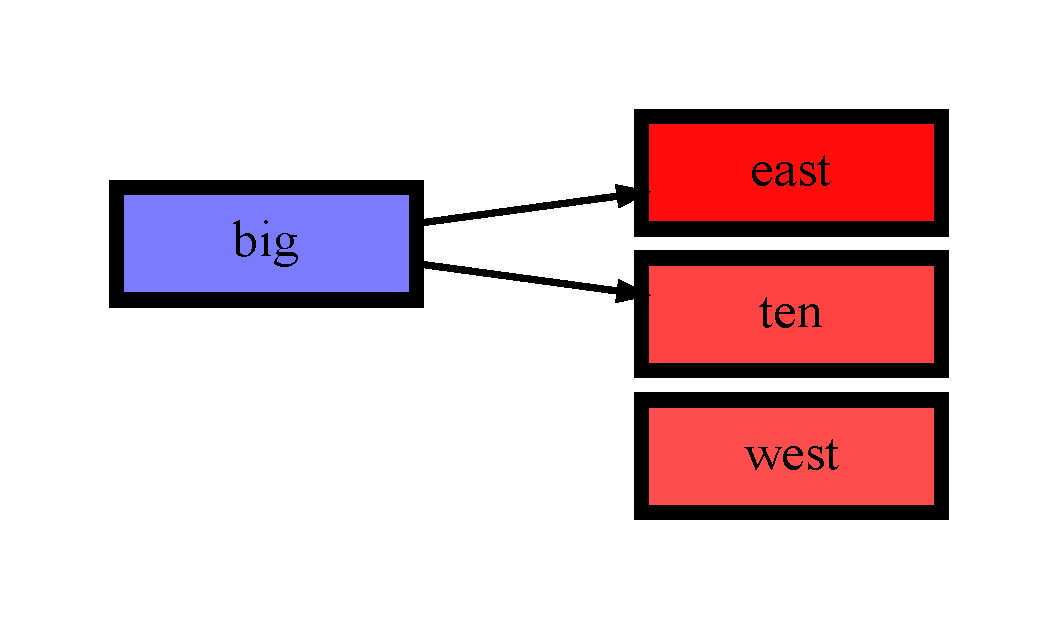
\includegraphics[height=0.7\textheight]{../images/gpt2-small_2_1817.pdf}
\end{frame}
\note{
    Is an automated interpretability method published last year by Alex Foote.
    Models a feature by building a syntactical graph based on a set of sample token strings.
    The point being that this model has an easily interpretable visualisation.
    Attempts to augment and prune these strings to find the simplest sufficient token patterns that activate the feature.
    
    Examples
}


\begin{frame}{Sparse Autoencoders} % 4 minutes
    \begin{align*}
        \vec y=&\mathrm{ReLU}\left(\mat W_e\vec x+\vec b\right)\\
        \hat{\vec x}=&\mat W_d\vec y\\
        \mathcal L(\vec x)=&\norm{\vec x-\hat{\vec x}}_2^2+\alpha\norm{\vec y}_1
    \end{align*}
    \centering
    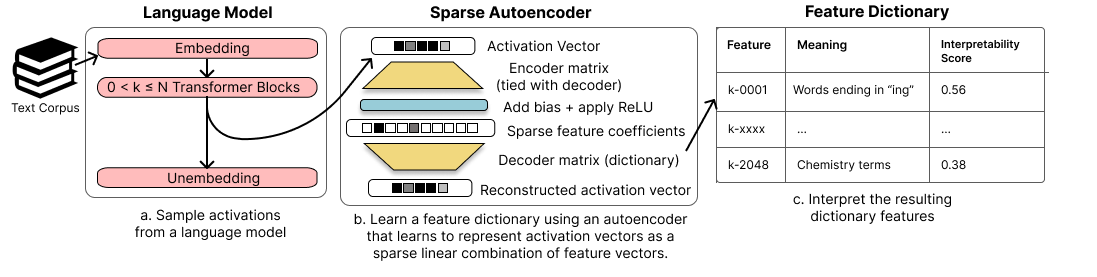
\includegraphics[height=0.5\textheight]{../images/cunningham_sae_illustration.png}
\end{frame}
\note{
    Neurons seem to be uninterpretable.
    Linear representation hypothesis -> We need to find the directions in MLP neuron space that are interpretable.
    SAEs are a method of doing this.
    Describe structure (and loss) of SAE with image and equations.
    Describe how it fits into the model.
}


\section{Method} % 8 minutes
\begin{frame}{Models and dataset} % 1 minute
    \begin{itemize}
        \item Language model: \texttt{gelu-1l}
        \item Dataset: \texttt{NeelNanda/c4-code-20k}
        \item SAE: \texttt{NeelNanda/sparse\_autoencoder/25.pt}
    \end{itemize}
\end{frame}
\note{
    In our experiments we use the same language model, dataset and SAE as in Neel Nanda's replication of the original Anthropic article.
    The language model is a single layer model.
    The dataset is a combination of code and text.

    Generalization from small LM and from early SAE.
}


\begin{frame}{Neuron2Graph} % 3 minutes
    \begin{itemize}
        \item Code based heavily on original implementation
        \item Refactored for readability and maintainability
        \item Original partial implementation in Rust to reduce memory and disk usage
    \end{itemize}
\end{frame}
\note{
    Original code is a rough translation of a Jupyter notebook.
    It is therefore very difficult to work with.
    We refactored it into a more maintainable form including a more modular structure and typing.
    This made our modifications easier to implement and test.
    Lastly, we also created a partial Rust implementation to reduce memory and disk usage.
    After training the N2Gs in Python, we convert them to the Rust implementation for storage and analysis.
}


\begin{frame}{Data sampling} % 3 minutes
    \begin{itemize}
        \item N2G originally used maximum activating samples
        \item We use a weighted random sampling approach
    \end{itemize}
    \begin{align*}
        w=&\e^{\alpha a}\\
        k=&\xi^{\frac1w}-[a<c]
    \end{align*}
\end{frame}
\note{
    N2G needs a set of samples that activate the feature.
    The original paper used maximum activating samples.
    This caused near-duplicates which contaminated the test set.
    Also other worries about maximum activating samples.
    We use a weighted random sampling approach.

    Explain the formulas.
}


\section{Results} % 9 minutes
\begin{frame}{Interpretability} % 3 minutes
    \only<1>{
    \begin{table}[ht]
        \centering
        \input{../images/figures/distribution_table.tex}
    \end{table}
    }
    \only<2>{
    \begin{figure}[ht]
        \centering
        
        \begin{subfigure}[b]{0.37\textwidth}
            \centering
            \includegraphics[width=\textwidth]{../images/figures/distribution_recall.pdf}
        \end{subfigure}
        \begin{subfigure}[b]{0.37\textwidth}
            \centering
            \includegraphics[width=\textwidth]{../images/figures/distribution_precision.pdf}
        \end{subfigure}
        \begin{subfigure}[b]{0.37\textwidth}
            \centering
            \includegraphics[width=\textwidth]{../images/figures/distribution_f1.pdf}
        \end{subfigure}
        \begin{subfigure}[b]{0.37\textwidth}
            \centering
            \includegraphics[width=\textwidth]{../images/figures/distribution_log_density.pdf}
        \end{subfigure}
    \end{figure}
    }
    \only<3>{
        \begin{figure}[ht]
            \centering
            
            \begin{subfigure}[b]{0.45\textwidth}
                \centering
                \includegraphics[width=\textwidth]{../images/figures/recall_precision_mlp.pdf}
                \caption{Recall vs Precision for MLP}
                \label{fig:recall_precision_mlp}
            \end{subfigure}
            \begin{subfigure}[b]{0.45\textwidth}
                \centering
                \includegraphics[width=\textwidth]{../images/figures/recall_precision_sae.pdf}
                \caption{Recall vs Precision for SAE}
            \end{subfigure}
        \end{figure}
    }
\end{frame}
\note{
    First slide:
    Table shows performance of N2G models on the two populations along with the feature densities, which we will come back to later.
    A two-sample bootstrap test shows that the means of the distributions are different for all statistics with $p<0.0001$.
    More interesting is the nuance in the distributions illustrated by these plots.

    Second slide:
    Look at performance metrics.
    Both populations seem to share a mode around 0, but SAE has second mode around 1.
    Indicates most are badly modelled, but some are very well modelled.
    To confirm this, we can look at...

    Third slide:
    We see that the recall and precision modes are generally aligned.
    }


\begin{frame}{Density} % 3 minutes
    \only<1>{
    \begin{figure}[ht]
        \centering
        \begin{subfigure}[b]{0.7\textwidth}
            \centering
            \includegraphics[width=\textwidth]{../images/figures/distribution_log_density.pdf}
        \end{subfigure}
    \end{figure}
    }
    \only<2>{
        \begin{figure}[ht]
            \centering
            \begin{subfigure}[b]{0.37\textwidth}
                \centering
                \includegraphics[width=\textwidth]{../images/figures/distribution_log_density.pdf}
            \end{subfigure}

    
            \begin{subfigure}[b]{0.37\textwidth}
                \centering
                \includegraphics[width=\textwidth]{../images/figures/density_f1.pdf}
            \end{subfigure}
            \begin{subfigure}[b]{0.37\textwidth}
                \centering
                \includegraphics[width=\textwidth]{../images/figures/f1_density.pdf}
            \end{subfigure}
        \end{figure}
    }
\end{frame}
\note{
    Explain density.

    First slide:
    As we saw before, the density distribution of the SAE features is bimodal, just like for the performance metrics.
    This raises the question of whether these modes are related.
    To investigate this, we can look at...

    Second slide:
    We partition the SAE features first by N2G F1 and then by density.
    While the low density cluster is not the same as the interpretable cluster, there is a clear relation.
    Indeed, the interpretable cluster is almost a subset of the low density cluster.
    In other words, all interpretable features have low density.
}


\begin{frame}{Geometry} % 3 minutes
    \only<1>{
        \begin{align*}
            \vec y=&\mathrm{ReLU}\left(\mat W_e\vec x+\vec b\right)\\
            \hat{\vec x}=&\mat W_d\vec y
        \end{align*}
    }
    \only<2>{
        \begin{table}[ht]
            \centering
            \input{../images/figures/direction_table.tex}
        \end{table}
    }
\end{frame}
\note{
    A last thing we will relate to these clusters is the geometry of the SAE latents.
    By "geometry", we mean the directions in MLP activation space that the SAE latents represent.
    Describe direction with reference to algebra.

    Second slide:
    To investigate these directions, we use cosine similarity and variance.
    Explain cosine similarity and variance.
    Explain table.
    We see that the high density cluster has over half of latents and very high cosine similarity.

    The rest has far lower cosine similarity (less than 1.9\%) but still far more than randomly chosen directions.
}


\section{Discussion} % 12 munutes
\begin{frame}{Results} % 5 minutes
    \begin{itemize}
        \item 
    \end{itemize}
\end{frame}
\note{

}


\begin{frame}{Methods} % 3 minutes
    
\end{frame}
\note{

}


\begin{frame}{Further Work} % 4 minutes

\end{frame}
\note{

}


\section{Conclusion} % 3 minutes
\begin{frame}{Conclusion} % 3 minutes
    
\end{frame}
\note{

}





\end{document}